\documentclass[a4paper,11pt]{article}
\usepackage{amsmath,amssymb,amsfonts}
\usepackage{graphicx}
\usepackage{textcomp}
\usepackage{xcolor}
\usepackage[margin=1in]{geometry}

% Set graphics path
\graphicspath{{../results/}}

\begin{document}

\title{\textbf{Semantic Communication over Noisy Channels: Joint vs. Separate Coding}}

\author{Author Name \\ Department \\ University/Organization \\ City, Country \\ email@domain.com}

\date{}
\maketitle

\begin{abstract}
In an era of exponentially growing data traffic, semantic communication offers a new paradigm: instead of transmitting every bit perfectly as dictated by Shannon's information theory, we aim to transmit only the underlying "meaning" of the information. In this paper, we present a semantic communication system for text based on the BERT language model. We compare two main approaches: a purely unsupervised semantic communication approach, where joint source-channel coding (JSCC) naturally learns to be robust to noise, versus a separation approach that utilizes classical Low-Density Parity-Check (LDPC) error correction. Our results demonstrate that under short block lengths and constrained bandwidth, the joint approach successfully preserves semantic meaning even in extreme noise conditions (SNR below -10 dB), leveraging redundancy in the semantic space as a natural channel code.
\end{abstract}

\textbf{Keywords:} Semantic Communication, Joint Source-Channel Coding, Deep Learning, LDPC

\section{Introduction}
Shannon's Separation Theorem states that under ideal conditions, with infinite block lengths, source coding (compression) and channel coding (error correction) can be designed independently without any loss of performance. However, in real-time systems with constrained block lengths, such as IoT communications or real-time media streaming, this theorem does not strictly hold.

Semantic Communication offers an alternative where the goal is not bit-level reconstruction of the input, but the delivery of meaningful content. Utilizing Deep Learning models, such as Large Language Models (LLMs), allows us to compress information into a low-dimensional bottleneck and transmit it over a channel.

In this project, we investigate whether a neural network trained jointly over a noisy channel (Joint Source-Channel Coding) outperforms a network trained over a clean channel that relies on agreed-upon mathematical error correction codes (LDPC), given the exact same physical bandwidth.

\section{Related Work}
\textit{Relevant papers on Semantic Communications, Joint Source-Channel Coding (JSCC), and the use of Autoencoders over communication channels will be integrated here (to be provided by the authors).}

\section{System Model}
The system comprises several mathematical components operating sequentially to form an end-to-end communication channel.

\subsection{The Semantic Encoder}
We map the input text $t$ into a continuous semantic space using a frozen BERT model, producing a vector $e \in \mathbb{R}^{768}$. This vector enters an Autoencoder that compresses it into a low-dimensional bottleneck $D$:
\begin{equation}
z = \sqrt{N P} \frac{f_\theta(e)}{\lVert f_\theta(e) \rVert_2}
\end{equation}
where $P$ is the average power per symbol $N = D/2$. Power normalization is necessary to establish a stable Signal-to-Noise Ratio (SNR).

\subsection{Quantization \& Straight-Through Estimator (STE)}
The continuous signal $z$ is quantized into a discrete 16-QAM constellation $\mathcal{C} = \{c_1, \dots, c_M\}$. During inference, the system selects the nearest point (Hard Assignment):
\begin{equation}
j_k^{\star} = \arg\min_{j} \lVert s_k - c_j \rVert_2^2, \qquad s_k^{\text{hard}} = c_{j_k^{\star}}
\end{equation}
During training, to allow gradients to flow back through this non-differentiable operation, we employ the Straight-Through Estimator (STE) with a soft assignment based on a temperature-weighted Softmax function:
\begin{equation}
w_{k,j} = \frac{\exp(-\sigma_q \lVert s_k - c_j \rVert_2^2)}{\sum_{l=1}^{M}\exp(-\sigma_q \lVert s_k - c_l \rVert_2^2)}, \qquad s_k^{\text{soft}} = \sum_{j=1}^{M} w_{k,j} c_j
\end{equation}
with an annealing hardness parameter $\sigma_q(t) = \min(\sigma_{\max}, \sigma_0 + \rho t)$. The gradient is passed via:
\begin{equation}
q_k = s_k^{\text{hard}} + \big(s_k^{\text{soft}} - \operatorname{sg}[s_k^{\text{soft}}]\big)
\end{equation}
Furthermore, to prevent mode collapse, we introduce a KL-Divergence penalty driving the empirical constellation usage $\hat{P}(c_j) = \frac{1}{B N} \sum_{b,k} w_{k,j}^{(b)}$ towards a uniform distribution $U(c_j) = 1/M$:
\begin{equation}
D_{\mathrm{KL}}\big(\hat P \| U\big) = \log M - H\big(\hat P\big)
\end{equation}

\subsection{AWGN Channel}
The compressed and quantized signal $q$ is transmitted through a channel that adds Additive White Gaussian Noise (AWGN):
\begin{equation}
r = q + n, \qquad n \sim \mathcal{N}(0, \sigma_n^2 I_D)
\end{equation}
The channel SNR in decibels is defined as:
\begin{equation}
\mathrm{SNR_{dB}} = 10 \log_{10}\frac{P}{\sigma_n^2}
\end{equation}

\subsection{Separation Baseline: LDPC Code}
For classical baseline comparison, we implemented a mechanism that converts the hard constellation indices to Gray-coded bits $\mathbf{u} \in \{0,1\}^K$ and encodes them using an LDPC generator matrix $G$ over GF(2) at a code rate $r = K/n = 1/2$:
\begin{equation}
\mathbf{x} = G^{\top}\mathbf{u} \bmod 2 \in \{0,1\}^n
\end{equation}
At the receiver, the noisy signals are translated into Log-Likelihood Ratios (LLRs) for each bit:
\begin{equation}
\Lambda_m = \log\frac{\Pr(x_m = 0 \mid r)}{\Pr(x_m = 1 \mid r)}
\end{equation}
which are decoded using the Belief-Propagation algorithm over the parity-check matrix $H$, such that $H\hat{\mathbf{x}} = \mathbf{0} \bmod 2$.

\section{Methodology}

\subsection{Unsupervised Semantic Compression}
The core methodological decision in this project was to \textbf{decouple the classification task from the compression process}.
The Autoencoder is trained to minimize the Mean Squared Error (MSE) reconstruction loss of the original BERT embedding:
\begin{equation}
\mathcal{L}_1(\theta, \phi) = \mathbb{E}_{e}\left[\big\lVert g_\phi(r) - e \big\rVert_2^2\right] + \lambda_{\mathrm{KL}} D_{\mathrm{KL}}\big(\hat P \| U\big)
\end{equation}
Only after the AE is trained and frozen do we train a classifier $h_\psi$ to predict the text category from the reconstructed BERT vector $\hat{e} = g_\phi(r)$ using label-smoothed Cross-Entropy Loss:
\begin{equation}
\mathcal{L}_2(\psi) = \mathbb{E}_{(e,y)}\left[ -\sum_{c=1}^{C} \alpha_c \tilde y_c \log \operatorname{softmax}(h_\psi(\hat{e}))_c \right]
\end{equation}
where $\tilde y_c = (1 - \varepsilon)\mathbb{1}[c = y] + \frac{\varepsilon}{C}$ and $\varepsilon$ is the label smoothing factor. This ensures that the transmitted information remains genuinely semantic and task-agnostic, rather than just task-specific "hints" for the 4-class categorization.

\textit{Note: For comparison, we also established an End-to-End model where the Encoder is optimized directly by the classification labels. While such a model achieves approximately 90\% accuracy under noise, it acts as a task-oriented system and loses the ability to reconstruct semantic meaning unrelated to the immediate classification task.}

\section{Experimental Results}

\subsection{Compression in a Clean Environment and the Semantic Illusion}
In a clean environment (SNR=20dB), as we decrease the bottleneck dimension, the fidelity to the original source decreases.

\begin{figure}[htbp]
\centering
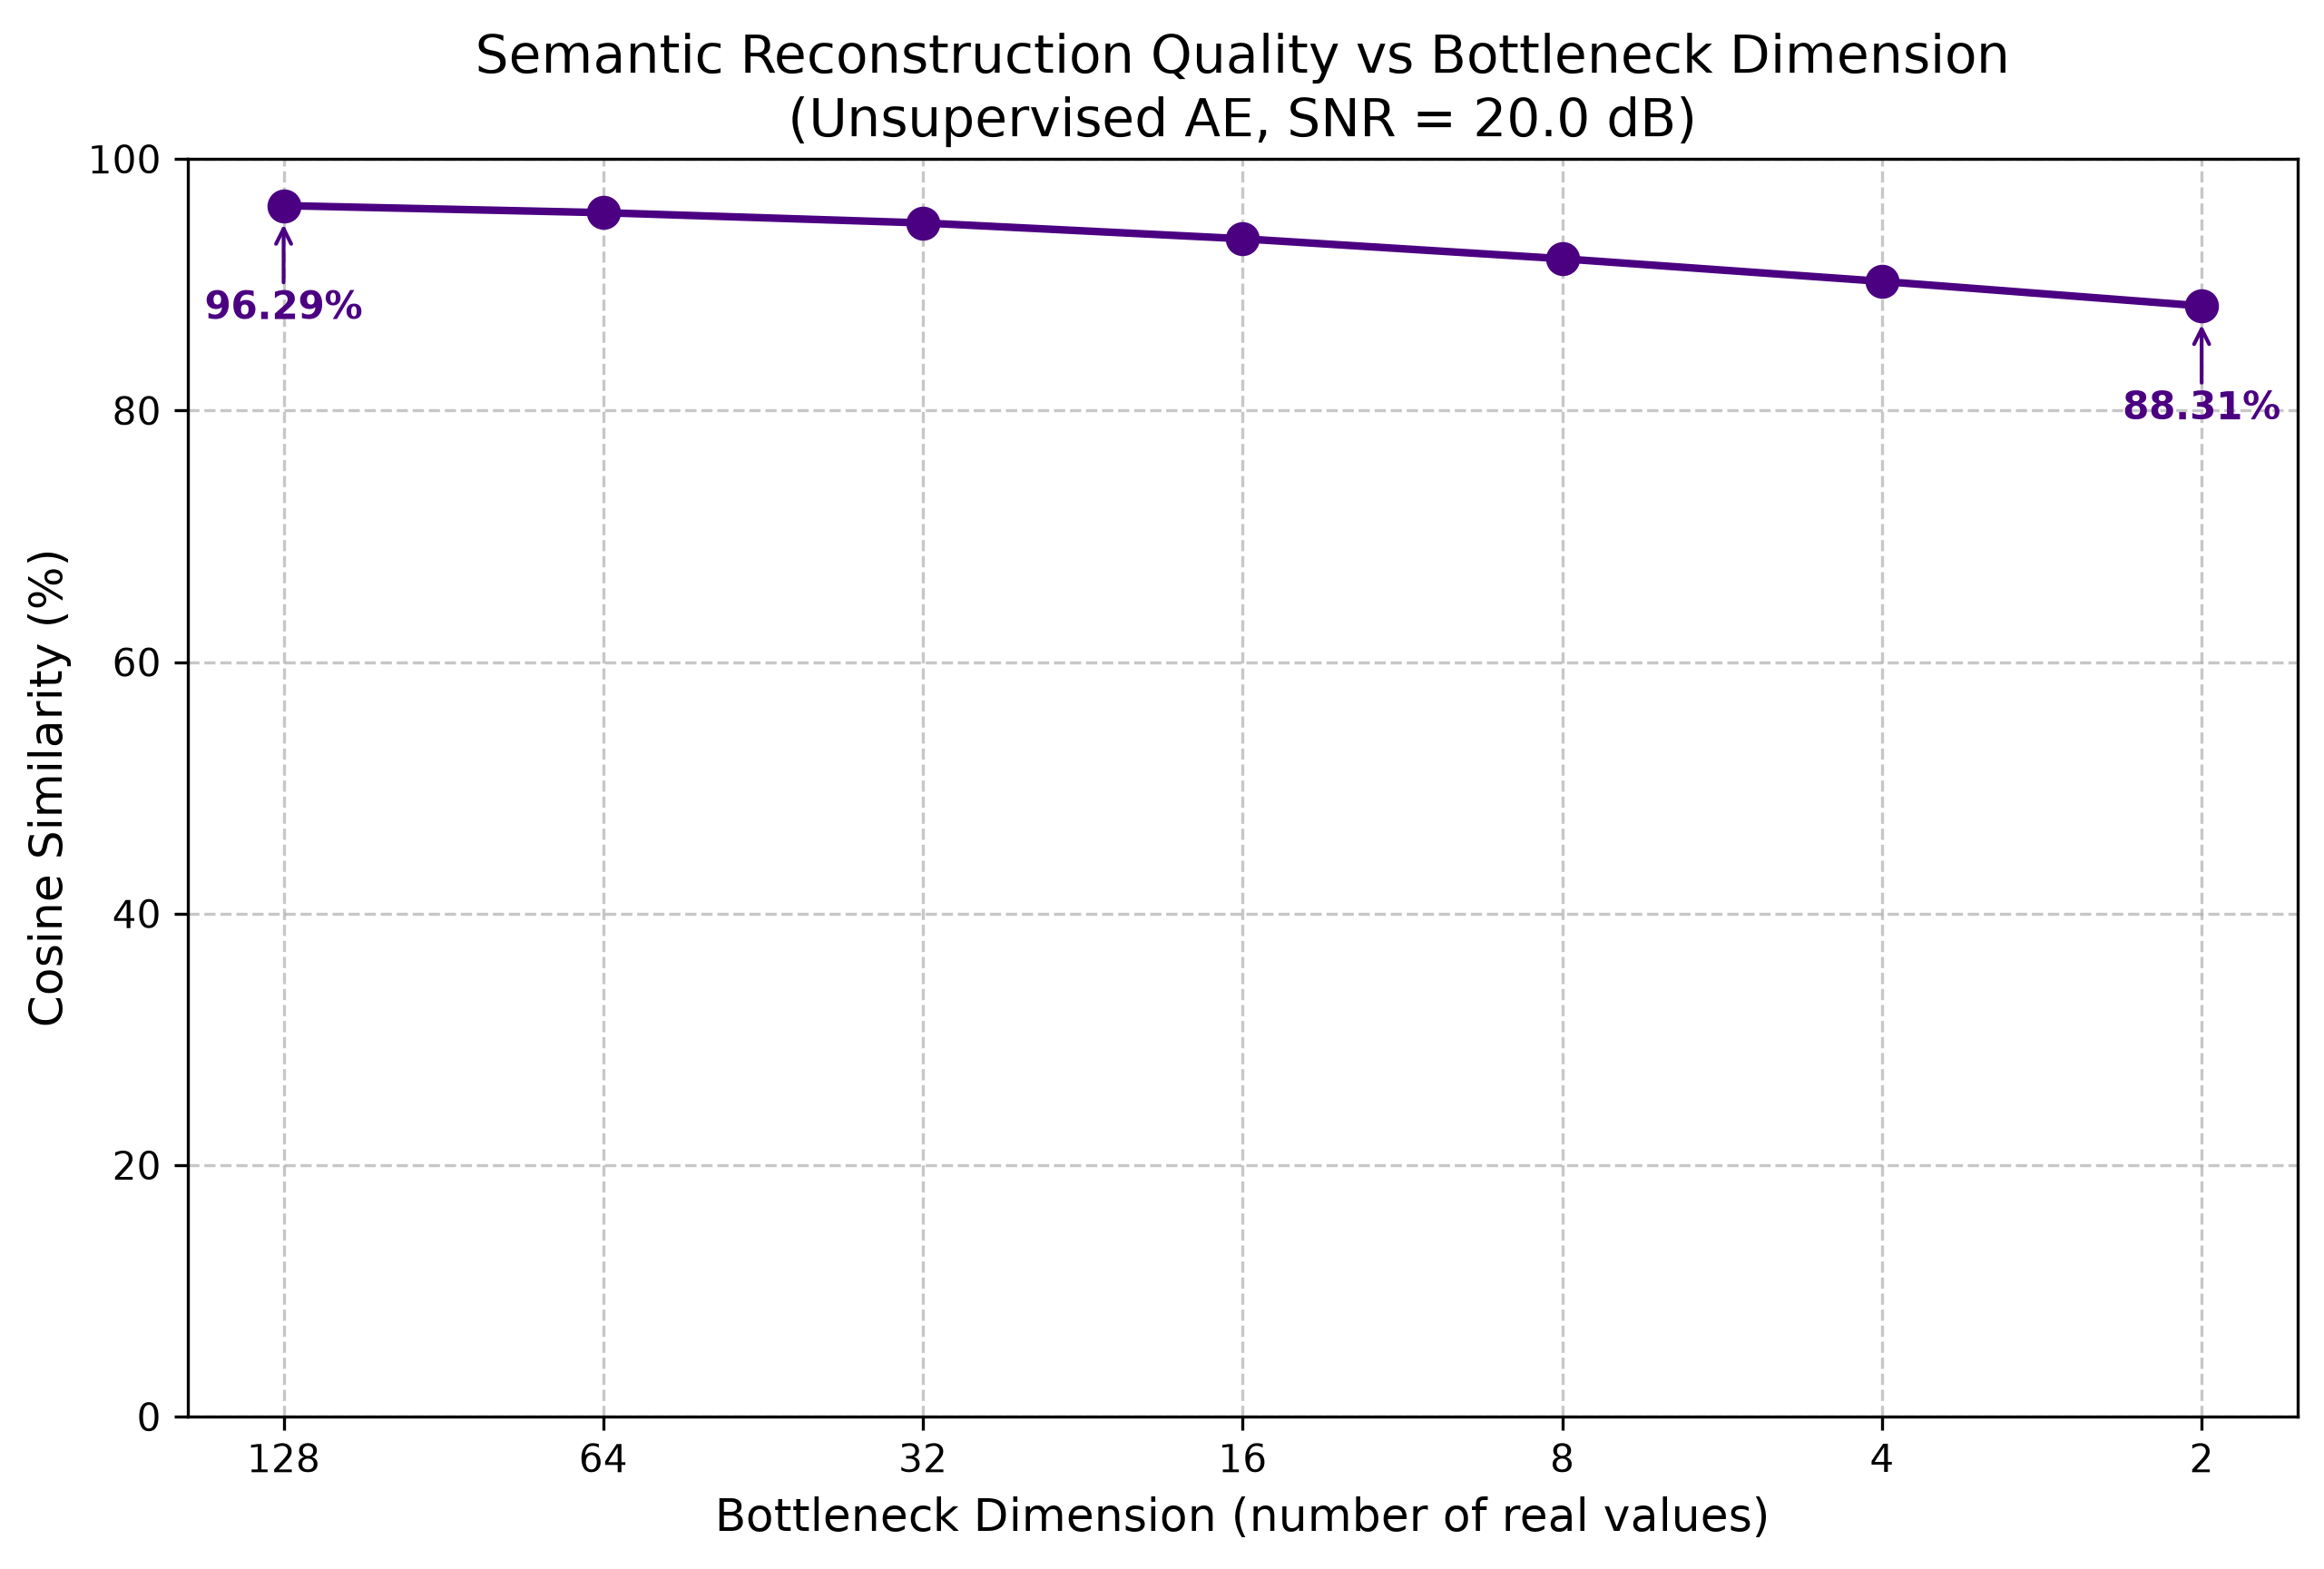
\includegraphics[width=0.8\textwidth]{dim_sweep/snr_20/reconstruction_plot.png}
\caption{Reconstruction fidelity across different bottleneck dimensions.}
\label{fig:recon}
\end{figure}

Even under extreme compression to 2 dimensions, the Cosine Similarity reconstruction is around 88.3\%. This might seem like high fidelity; however, the similarity between any average sentence and a random sentence in the dataset is roughly 85.98\%. This baseline "illusion" explains the sharp drop in classification accuracy to 64.9\% at these dimensions.

\begin{figure}[htbp]
\centering

\includegraphics[width=0.8\textwidth]{dim_sweep/snr_20/dim_sweep.png}
\caption{Classification accuracy across bottleneck dimensions in a clean channel.}
\label{fig:dim20}
\end{figure}

\subsection{Noise Robustness through High Redundancy}
When fixing the compression to 64 dimensions (allowing excellent semantic transfer), we observe how the system handles increasing noise. Even at -10 dB, where the noise energy is 10 times stronger than the signal energy, the channel-aware model extracts enough meaning to maintain an accuracy of 53.6\%. The redundancy in higher dimensions serves as a naturally learned channel error-correction code.

\begin{figure}[htbp]
\centering
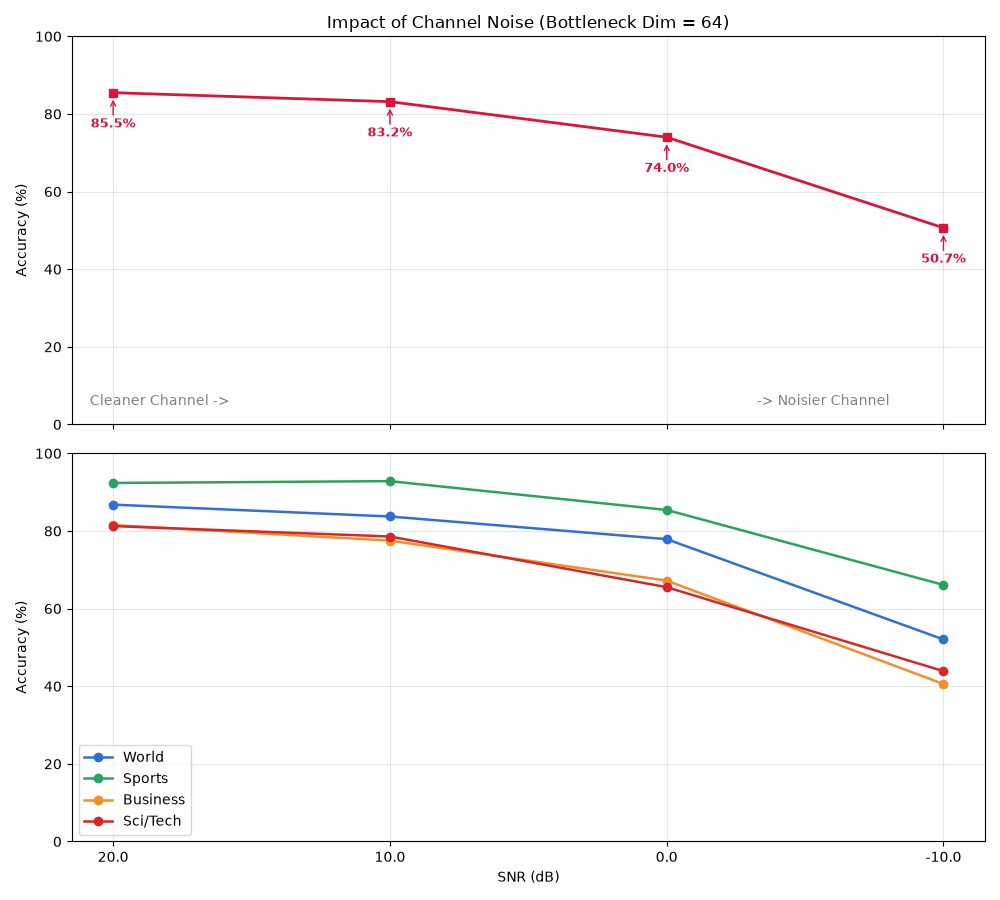
\includegraphics[width=0.8\textwidth]{snr_sweep/dim_64/snr_sweep.png}
\caption{System performance across varying SNR levels with a fixed 64D bottleneck.}
\label{fig:snrsweep}
\end{figure}

\subsection{SNR Mismatch Penalty}
An experiment evaluating a single model trained at SNR=10dB across varying noise levels highlighted the necessity of dedicated training. The model completely collapsed (37.6\% accuracy) at extreme noise (-10dB), whereas an identical model pre-trained for that specific environment exhibited much higher resilience. This proves the critical need for continuous Channel Estimation.

\begin{figure}[htbp]
\centering
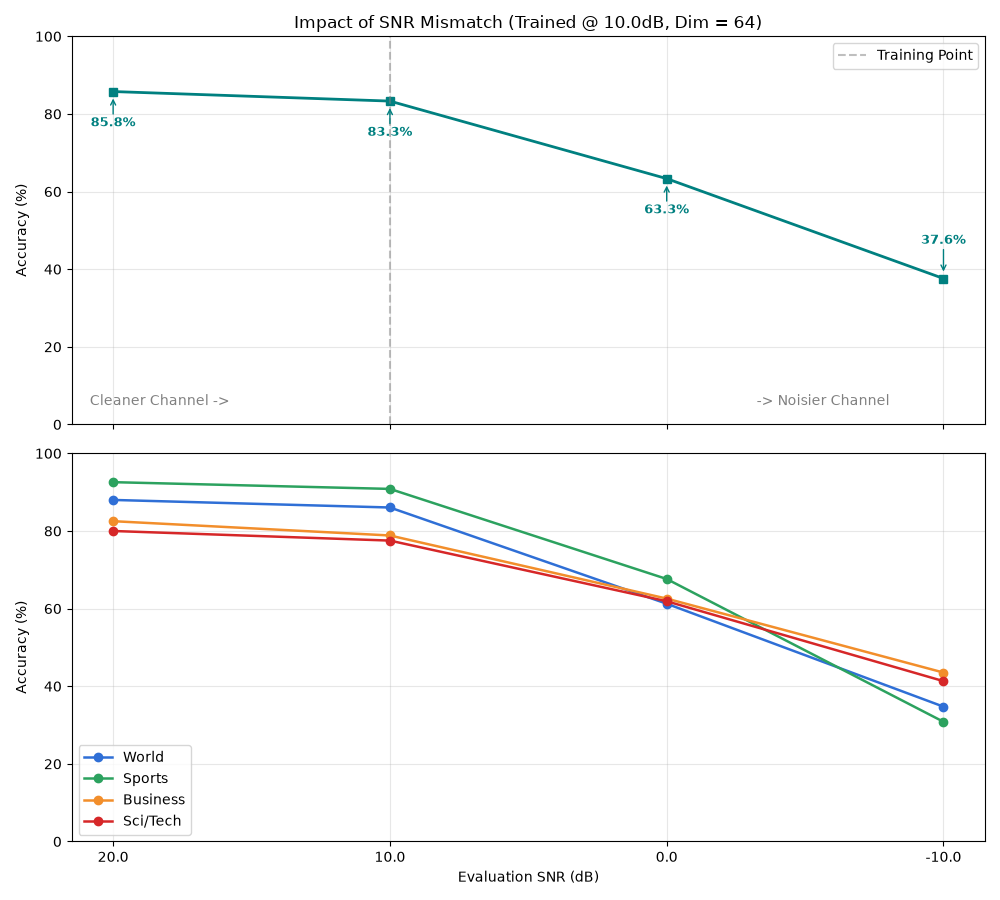
\includegraphics[width=0.8\textwidth]{mismatch_sweep/train_snr_10_dim_64/mismatch_sweep.png}
\caption{SNR Mismatch penalty: performance of a model trained at 10dB across other noise levels.}
\label{fig:mismatch}
\end{figure}

\subsection{Joint vs. Separate Source-Channel Coding}
\textit{(The final comparison graph showcasing the differences between Joint JSCC and Separate coding with LDPC over the same bandwidth footprint will be presented here).}

\section{Conclusion}
The research results prove that semantic communication allows the transfer of meaning over highly hostile channels. The Joint Source-Channel Coding approach successfully learns stable representations against noise. The bottleneck dimension serves a dual purpose: a vessel for delicate semantic details and a physical safety margin (redundancy) to compensate for channel noise.

Future work could include replacing the current Quantizer with advanced VQ-VAE approaches, transitioning to larger generative models, and integrating multi-user communication (MIMO).

\end{document}
